\section{Model and spatial correction}
\subsection{Interface motion and force channels}
Three fractions $\phi_i$, $i\in\{0,1,2\}$, satisfy
\begin{equation}
 \ph\in\mathcal D=\{\ph:\ \phi_i\geq0,\quad \textstyle\sum_i\phi_i=1\}.
 \label{eq:simplex}
\end{equation}
Phase 0 consumes grains 1 and 2. The target binary-interface law is
\begin{equation}
 v_n=M_{ij}(\Delta f_{ij}-\gamma_{ij}\kappa),
 \label{eq:sharp}
\end{equation}
with normal and curvature signs fixed consistently with the ordered pair. Here $\gamma_{ij}$ is interfacial energy, $M_{ij}$ mobility and $\Delta f_{ij}=-\Delta f_{ji}$ bulk driving force. The junction satisfies interfacial force balance. We use the translating-junction and grain-consumption references associated with Hoffrogge et al.\ \citep{hoffrogge2025}.

In the benchmark's B2 formulation, the force separates into capillary and bulk channels,
\begin{equation}
 R_i=C_i+B_i
 =\sum_{j\ne i}^{\mathrm{active}}M_{ij}
 [-\gamma_{ij}K_{ij}+J_{ij}+b_{ij}\Delta f_{ij}],
 \label{eq:b2}
\end{equation}
where
\begin{align}
 K_{ij}&=\frac{1}{N_a}\left[\Delta_h\phi_j-\Delta_h\phi_i+
 \frac{\pi^2}{\eta^2}(\phi_j-\phi_i)\right],\label{eq:K}\\
 J_{ij}&=\frac{1}{N_a}\sum_{k\ne i,j}^{\mathrm{active}}
 (\gamma_{jk}-\gamma_{ik})
 \left(\Delta_h\phi_k+\frac{\pi^2}{\eta^2}\phi_k\right),\label{eq:J}\\
 b_{ij}&=\frac{\pi}{\eta}(\phi_i+\phi_j)\sqrt{\phi_i\phi_j}.
 \label{eq:b}
\end{align}
The interface width is $\eta$. A phase is eligible at a node when its fraction is positive or its discrete Laplacian is nonzero. The count $N_a$ divides $K$ and $J$, not the complete pair sum again. Each unordered eligible pair supplies equal and opposite phase increments. These discrete choices specify our implementation; they do not assert executable identity with Pace3D or MICRESS.

The binary profile is a clipped sine across a band of width $\eta$,
\begin{equation}
 \phi_i(d)=
 \begin{cases}
 0,&d\leq-\eta/2,\\
 \tfrac12[1+\sin(\pi d/\eta)],&|d|<\eta/2,\\
 1,&d\geq\eta/2 ,
 \end{cases}
 \qquad\phi_j=1-\phi_i .
 \label{eq:profile}
\end{equation}
The oriented coordinate $d$ and the case-specific initial fields are specified in the Supplementary Material. All tests use common positive pair mobility.

\subsection{A multiplier from neighboring ternary support}
Define
\begin{equation}
 P(\mathbf x)=27\phi_0(\mathbf x)\phi_1(\mathbf x)\phi_2(\mathbf x).
 \label{eq:product}
\end{equation}
On the simplex, $0\leq P\leq1$, with equality at one for equal fractions. A square maximum filter extends the signal over radius $\rho$:
\begin{equation}
 H_\rho(\mathbf x)=
 \max_{\|\mathbf y-\mathbf x\|_\infty\leq\rho}
 [(1-S(\mathbf y))P(\mathbf y)],\qquad m=1+\chi H_\rho .
 \label{eq:halo}
\end{equation}
The whole correction sets $S=0$ everywhere. The corrected force and constrained step are
\begin{align}
 \widetilde R_i&=mC_i+B_i,\label{eq:corrected}\\
 \ph^{n+1}&=\Pi_{\mathcal D}
 [\ph^n+\Dt_{\rm raw}\widetilde{\mathbf R}(\ph^n)] .
 \label{eq:step}
\end{align}
The reference code evaluates the equivalent force by adding $\chi H_\rho$ times the capillary contribution to the native force. The developed-front comparison retains its original Euclidean simplex projector; later cold calculations use a roundoff-safe implementation (Supplementary material).

The baseline prescription is $\chi=27$ and $\rho=\eta$, with an integer cell radius on each tested grid. These are empirical operating values, not outputs of an asymptotic matching formula or a fit repeated for each test. Four one-factor perturbations are reported in Section~\ref{sec:robustness}.

Figure~\ref{fig:method_schematic} summarizes the source, neighborhood extension and force-channel modification.
\begin{figure}[tbp]
 \centering
 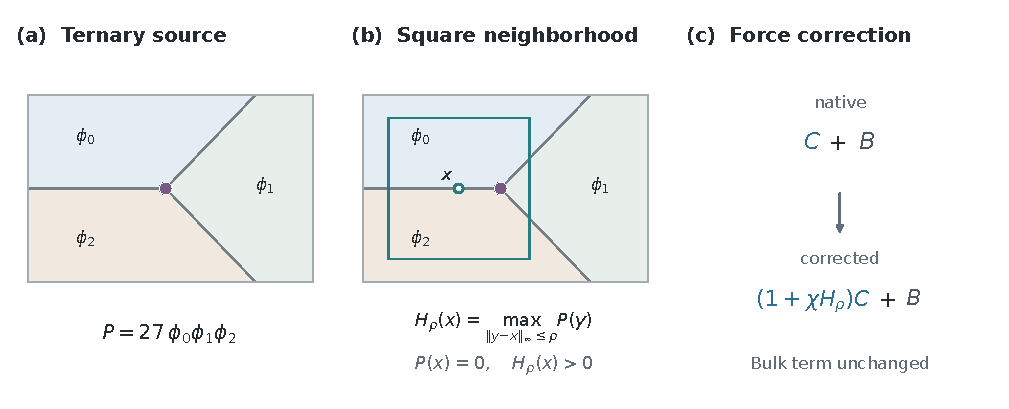
\includegraphics[width=0.96\linewidth]{method_schematic.pdf}
 \caption{Illustrative, not simulation-derived or to scale. (a) The source signal is $P=27\phi_0\phi_1\phi_2$. (b) The thin teal square is the width-$2\rho$ sampling region $\|y-x\|_\infty\leq\rho$, centered at binary receiver $x$ and containing the source: $P(x)=0$ but $H_\rho(x)>0$ (whole correction, $S=0$). (c) $(1+\chi H_\rho)$ weights capillary $C$ only; bulk $B$ is unchanged. No core angle is measured or implied.}
 \label{fig:method_schematic}
\end{figure}

A globally binary field has $P\equiv0$ and hence $H_\rho\equiv0$: the binary calibration problem is unchanged. A binary node near a junction can nevertheless receive a nonzero halo from neighboring ternary support. Source localization and output localization are therefore different. The multiplier satisfies $1\leq m\leq1+\chi$, but that bound is not a stability or accuracy guarantee.

Equation~\eqref{eq:corrected} changes the relative capillary and bulk forces. At a forced balance $\mathbf C+\mathbf B=0$, the corrected force becomes $(1-m)\mathbf B$, which need not vanish. The correction is consequently distinct from a uniform mobility or time change and is assessed against sharp-interface observables.

\subsection{Local memory after neighborhood overlap}
The optional memory variant suppresses selected ternary sources after correction neighborhoods overlap. At controller evaluations, label the eight-connected components of $\{P>0\}$. Components are incident when their radius-$\rho$ square dilations intersect. All components incident to an overlap are marked for suppression. A current component inherits suppression if it touches the preceding suppressed support dilated by one grid cell. Inheritance is updated after every Euler step, while new overlap is checked only at the prescribed controller times.

The stored object is a spatial support mask, not a permanent label number. Suppression removes sources before maximum filtering in Eq.~\eqref{eq:halo}; a nearby unsuppressed component can still contribute. This is a discrete history rule rather than a physical material-lineage model. It requires exact absent-phase values. Positive tails would change support topology and need a separately qualified construction. The exact label-window algorithm is given in the Supplementary Material.

\section{Benchmark design and measurements}
Lengths are normalized by strip width $W$, and time by $W^2/(M_0\gamma_0)$. The normalized pair energies are $\gamma_{01}=\gamma_{02}=1$, $\gamma_{12}=q$. For negative drive parameter $p$, the entries $\Delta f_{01}=\Delta f_{02}=-p>0$ favor phase 0; the grain--grain bulk force is zero. The equilibrium opening angle is $2\arccos(q/2)$.

The translating-front case uses $q=\sqrt3$, $p=-50$ and a $W\times4W$ moving domain. Matched runs begin from a common developed field and cover a further time of $0.25$. A separate cold comparison includes each route's binary calibration and junction evolution. The interacting case uses $q=1.5$, $p=-30$ and a $W\times24W$ domain containing junction pairs with nominal separations $7W$ and $10W$. Its comparison horizon is $0.12$. Outer boundaries have zero normal gradients.

For the cold controlled comparisons, a separate binary planar calculation fixes each recipe's clock factor
\begin{equation}
 a=V_{\rm target}/V_{\rm planar},\qquad t=s/a ,
 \label{eq:clock}
\end{equation}
where $s$ is raw solver time. This is the time coordinate corresponding to a uniform factor $a$ on the whole right-hand side. It is used for observation and controller scheduling, and is not fitted to junction outputs. Calibration is repeated if the stencil, grid, width or raw timestep changes. The original matched developed-front comparison retains the common nominal solver clock.

Migration speeds are fitted to interface-position and phase-area histories in settled windows. The translating-front shape is reconstructed at the same 92 physical transverse positions, interpolated before maximum alignment. Its RMS error is
\begin{equation}
 e_{\RMS}=\left[\frac1{92}\sum_{\ell=1}^{92}
 (\widehat y_h(x_\ell)-\widehat y_\star(x_\ell))^2\right]^{1/2}.
 \label{eq:rms}
\end{equation}
Alignment removes translation; this is not absolute-position error.

For grain consumption, marching-squares boundaries are compared in physical coordinates using symmetric Hausdorff distance
\begin{equation}
 \HH(\Gamma_h,\Gamma_\star)=
 \max\left\{\sup_{\mathbf x\in\Gamma_h}\inf_{\mathbf y\in\Gamma_\star}|\mathbf x-\mathbf y|,
 \sup_{\mathbf y\in\Gamma_\star}\inf_{\mathbf x\in\Gamma_h}|\mathbf x-\mathbf y|\right\}.
 \label{eq:hausdorff}
\end{equation}
Segment sampling supplies a distance bracket; it does not enclose continuum-model error. Disappearance time $T_{99}$ is bracketed when reconstructed grain area first falls to 1\% of its initial sharp-reference area. A boundary absent before its reference disappears is recorded as an empty-boundary outcome, never as zero error.

The operational accuracy targets are 5\% speed error and $0.05W$ shape error. They are study choices, not universal criteria. Settling uses early/late speed fits and aligned-profile changes; fraction bounds and the unit-sum constraint are checked separately. Numerical settings, schedules and reconstruction details are supplied in the Supplementary Material.
